%&"../main"
\documentclass[../main]{subfiles}
\begin{document}

\chapter{电磁波参量的测定实验}%
\label{cha:电磁波参量的测定实验}

\section{实验目的}%
\label{sec:\arabic{chapter}实验目的}

\begin{enumerate}

	\item 观察电磁波的传播特性;

	\item 通过测定自由空间中电磁波的波长$ \lambda $,来确定电磁波传播的相位
		常数$ k $和传播速度$ v $;

	\item 了解用相干波的原理测量波长的方法。

\end{enumerate}

\section{实验内容}%
\label{sec:\arabic{chapter}实验内容}

\begin{enumerate}

	\item 了解并熟悉电磁波综合测试仪的工作特点、线路结构、使用方法;

	\item 测量信号源的工作波长(或频率)。

\end{enumerate}

\section{实验原理与说明}%
\label{sec:\arabic{chapter}实验原理与说明}

\subsection{所使用的实验仪器}%
\label{sub:\arabic{chapter}所使用的实验仪器}

\begin{table}[htbp]
	\centering
	\caption{实验仪器}
	\label{tab:\arabic{chapter}实验仪器}
	\csvautobooktabular{tab/1/BOM.csv}
\end{table}

实验仪器布置图如图\ref{fig:实验仪器布置图}所示。

\begin{figure}[htbp]
	\centering
	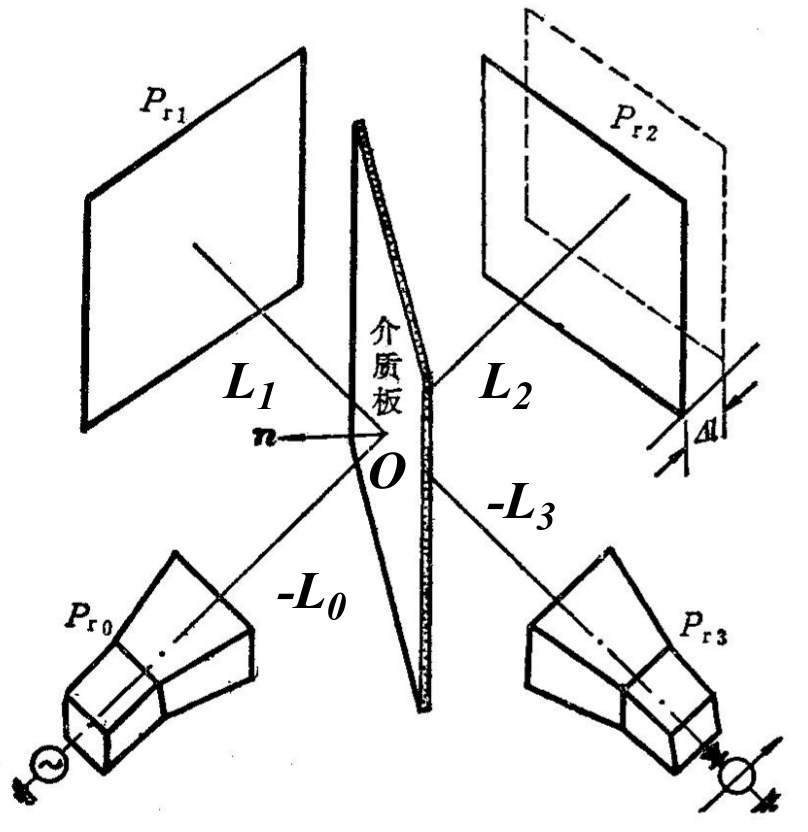
\includegraphics[width = 0.8\linewidth]{1/experiment.png}
	\caption{实验仪器布置图}
	\label{fig:实验仪器布置图}
\end{figure}

固态信号源所产生的信号经可变衰减器至矩形喇叭天线,在接收端用矩形喇叭天线接收信号
,接收到的信号经晶体检波器后通过微安表指示。

频率——测微器刻度对照表如表\ref{tab:频率——测微器刻度对照表}所示。

\begin{table}[htbp]
	\centering
	\caption{频率——测微器刻度对照表}
	\label{tab:频率——测微器刻度对照表}
	\csvautobooktabular{tab/1/freq.csv}
\end{table}

\subsection{原理}%
\label{sub:\arabic{chapter}原理}

本实验利用相干波原理,通过测得的电磁波的波长$ \lambda $, 再由关系式\ref{eq:k}和
\ref{eq:v}得到电磁波的主要参量$ k $,$ v $等。

\begin{align}
	\label{eq:k}
	k & = \dfrac{2\pi }{\lambda }\\
	\label{eq:v}
	v & = \lambda f = \dfrac{\omega }{k}
\end{align}

实验示意图如图\ref{fig:实验示意图}所示。图中$ P_\mathrm{r0}, P_\mathrm{r1},
P_\mathrm{r2}, P_\mathrm{r3} $分别表示辐射喇叭、固定反射板、可动反射板和接收喇叭
,图中介质板是一\SI{30x30}{\mm} 的玻璃板,它对电磁波进行反射、折射后,可实
现相干波测试。

\begin{figure}[htbp]
	\centering
	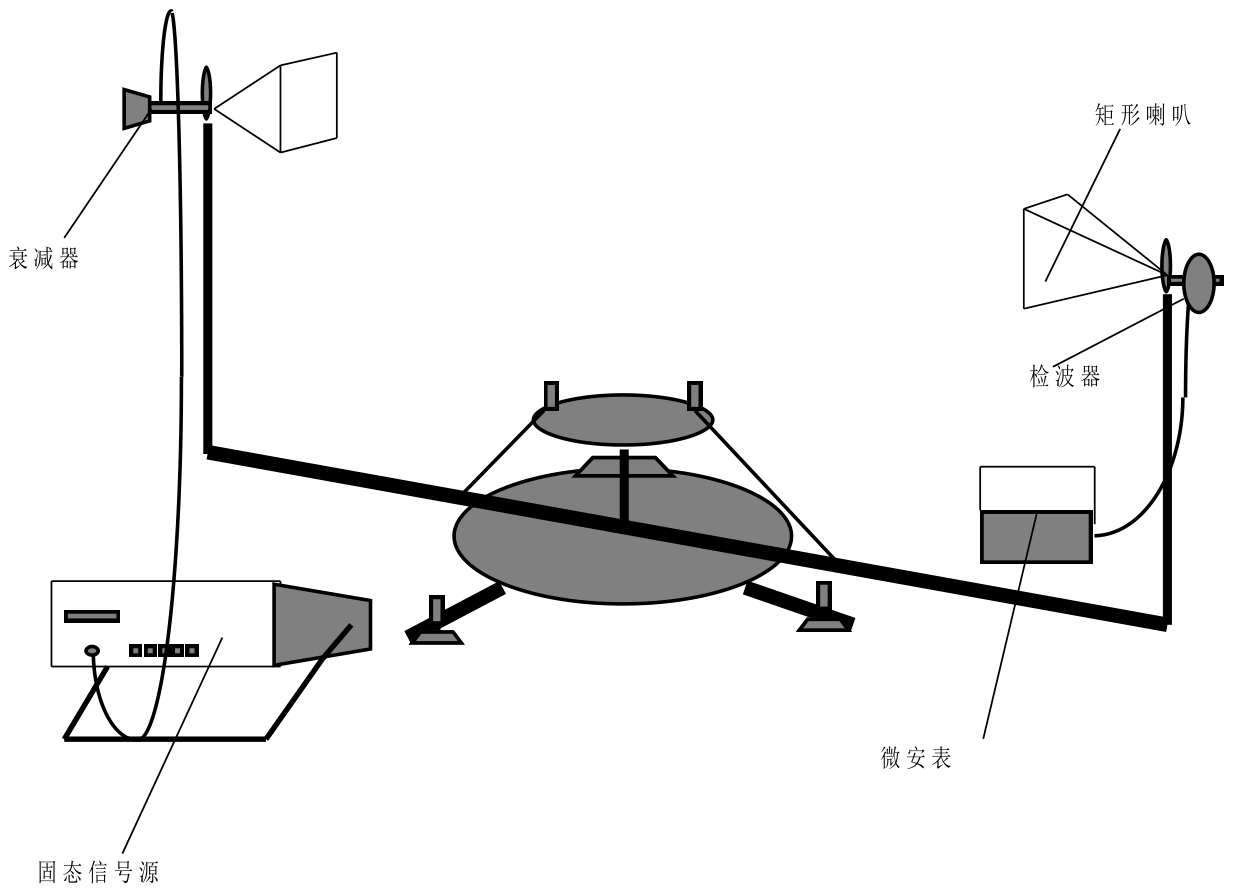
\includegraphics[width = 0.8\linewidth]{1/instruction.png}
	\caption{实验示意图}
	\label{fig:实验示意图}
\end{figure}

当入射波以入射角$ \theta $向介质板斜投射时,在分界面上产生反射波$ \vec{E}^- $
和折射波$ \vec{E}' $ 。设入射波为垂直极化波,用$ R $表示介质板的反射系数,用$ T
$分别表示由空气进入介质板再进入空气后的折射系数,$ R $与$ T $为复数。另外固定的和可动
的金属反射板的反射系数均为-1。

假设发射的平面波为:

\begin{align}
	E^+ = E^0 e^{-\jmath kl}
\end{align}

分析时$ l $为在喇叭天线$ P_\mathrm{r0} $发射的波的传播方向上与相位参考零点所在的
面之间的距离(有正、负值之分),相位参考零点不妨选介质板的中心点。忽略介质板与金属
板之间的多次作用效应,则在反射板1与反射板2处的入射场$ E^+ $与反射场$ E^- $可表示
为:

\begin{align}
	E_1^+ & = RE^0 \exp(-\jmath kl) |_{l = L_1}\\
	E_1^- & = -RE^0 \exp\big(\jmath k(l - 2L_1)\big) |_{l = L_1}\\
	E_2^+ & = TE^0 \exp(-\jmath kl) |_{l = L_2}\\
	E_2^- & = -TE^0 \exp\big(\jmath k(l - 2L_2)\big) |_{l = L_2}
\end{align}

它们在接收喇叭$ P_\mathrm{r3} $处的场为:

\begin{align}
	E_1^- & = -RE^0 \exp\big(\jmath k(l - 2L_1)\big) |_{l = L_3}\\
	E_2^- & = -TE^0 \exp\big(\jmath k(l - 2L_2)\big) |_{l = L_3}
\end{align}

由于它们同频同极化,它们相干合成的场可写为

\begin{align}
	\label{eq:E}
	E & = E_1^- + E_2^- = TRE^0\exp\big(\jmath k(-L_3 - 2L_1)\big) - RTE^0
	\exp\big(\jmath k(-L_3 - 2L_2)\big)\\
	  & = TRE^0\exp(-\jmath kL_3)\big(\exp(-2\jmath kL_1) + \exp(-2\jmath
	  kL_2)\big)\\
	  & = A \big(1 + \exp(-\jmath 2k\Delta l)\big)
\end{align}

其中

\begin{align}
	A & = -TRE^0\exp(-\jmath kL_3)\exp(-\jmath k 2L_1)\\
	\Delta l & = L_2 - L_1
\end{align}

上述过程可以用图\ref{fig:波形图}来示意。

\begin{figure}[htbp]
	\centering
	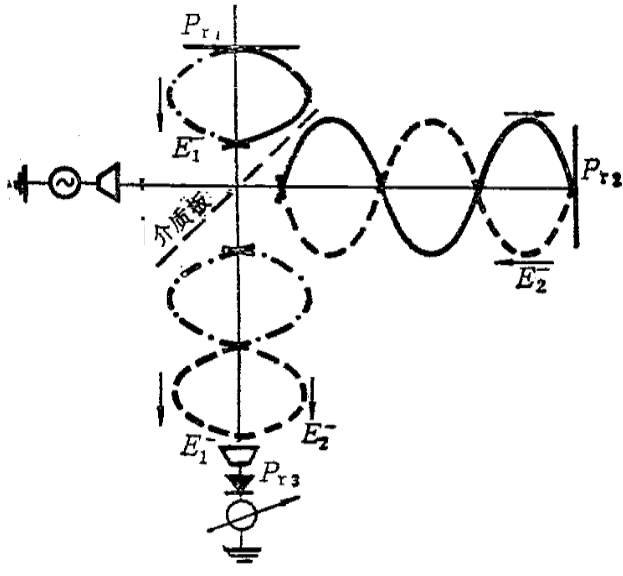
\includegraphics[width = 0.8\linewidth]{1/wave.png}
	\caption{波形图}
	\label{fig:波形图}
\end{figure}

测量时,由于被测场$ E $处于测试结构的近区场范围内,不完全满足理想平面波的特性,
这不仅影响着零点位置均匀分布,而且使波幅值也有起伏。为了测准波长$ \lambda $值,
一般采用$ P_\mathrm{r3} $为零指示办法。由式\ref{eq:E}可发现,合成波中当$ \exp(
-\jmath 2k\Delta l ) = - 1 $时,$ P_\mathrm{r3} $处的场为零。实验时,固定$ L_0,
L_1, L_3 $移动$ L_2 $,使得$ P_\mathrm{r3} $处的场为零。这时可得条件

\begin{align}
	\exp( - \jmath 2k\Delta l) & = - 1\\
	2k\Delta l_n & = (2n + 1)\pi\\
	\Delta l_n & = \dfrac{2n + 1}{4}\lambda \\
	\label{eq:lambda}
	L_{2n} - L_1 & = \dfrac{2n + 1}{4}\lambda
\end{align}

不难发现相邻两个零值的 $ L_{2n} $与 $ L_{2n + 1} $ 之间的间距为 $ \dfrac{\lambda
}{2} $ ,从而达到测量目的。

$ n = N, L_{2N} - L_1 = \dfrac{2(i + N) + 1}{4}\lambda $得$ N + 1 $个零点位置
$L_{2N} $可见,当零点总数为$ (N + 1) $时,$ P $上移动的总距离为$ L_{2N} - L_{20}
$,它相当于$ N $个半波长数。即:$ 2L_{2N} - L_{20} = N\lambda $,故:
$ \lambda = 2\dfrac{L_{2N} - L{20}}{N} $。根据式\ref{eq:k}和\ref{eq:v} 就可得到
所测电磁波的参量$ \lambda , k, v $等值。可见测试波长$ \lambda $所用公式得出的是
平均值。从理论上讲,$ n $值越大,测出的$ \lambda $值精度应越高。实际测试时,一般
取$ n = 4 $已足够,这时相应于 5 个波节点,所测的波长为

\begin{align}
	\lambda = 4\dfrac{L_{24} - L_{20}}{4}
\end{align}

它表示了 5 个波节点的距离$ L_{24} - L_{20} $,相应于 4 个半波长。

\section{实验步骤}%
\label{sec:\arabic{chapter}实验步骤}

\begin{enumerate}

	\item 了解并熟悉电磁波综合测试仪的工作特点、线路结构、使用方法;

	\item 测量电磁波的波长;首先调整好电磁波综合测试仪使能进行正常工作。然后
		测出电磁波的波长,根据测出的值,得到电磁波的重要参量$ k $,由$ k
		$值可计算出传播速度;

		\begin{align}
			v = \dfrac{2\pi f}{k} = \dfrac{1}{\sqrt{\mu_0\varepsilon_0}} = c
		\end{align}

	\item 用波长计(或频率计)测出信号源的工作波长(或频率)。把测试值填入表
		\ref{tab:电磁波参量测试数据表}中。如采用\SI{3}{\cm}标准信号源,
		则可改变信号源工作频率$ f_0 $(即改变$ \lambda_0 $)。由以上实验
		内容,得到相应的电磁波参量$ \lambda, k, v $,并与$ \lambda_0,
		k_0, v_0 $ 作比较(如使用该仪器本身的固态信号源,它已调定在一个
		固定频率$ f_0 $上工作,故$ ν $及$ k $不能改变)。

\end{enumerate}

\begin{table}[htbp]
	\centering
	\caption{测试数据}
	\label{tab:测试数据}
	\csvautobooktabular{tab/1/measure.csv}
\end{table}

\begin{table}[htbp]
	\centering
	\caption{电磁波参量测试数据表}
	\label{tab:电磁波参量测试数据表}
	\csvautobooktabular{tab/1/data.csv}
\end{table}

\section{实验结果}%
\label{sec:\arabic{chapter}实验结果}

实验数据见表\ref{tab:测试数据},实验结果见表\ref{tab:电磁波参量测试数据表}。一共
在\SI{20}{\uA}的位置测量了6组数据,求平均后得到3组零点时的长度,利用式
\ref{eq:lambda}, \ref{eq:k}和\ref{eq:v}求出$ \lambda, k, v $。2次测量相对误差为
0.9067\%和0.9592\%。

\section{讨论}%
\label{sec:\arabic{chapter}讨论}

测量6组数据得到3组零点时的长度$ l_1, l_2, l_3 $,每2个相邻零点的长度差为一个半波
长$ \dfrac{\lambda_1 }{2} = l_2 - l_1 $。对这2个半波长求平均是不合理的,因为如式
\ref{eq:lambda1}:

\begin{align}
	\dfrac{\lambda_1}{2} & = l_2 - l_1\\
	\dfrac{\lambda_2}{2} & = l_3 - l_2\\
	\dfrac{\lambda }{2} & = \dfrac{1}{2}\Big(\dfrac{\lambda_1}{2} +
	\label{eq:lambda1}
	\dfrac{\lambda_2}{2}\Big)\\
			    & = \dfrac{l_2 - l_1 + l_3 - l_2}{2}\\
			    & = \dfrac{l_3 - l_1}{2}
\end{align}

会导致$ l_2 $的数据无效。好的办法应该是式 \ref{eq:lambda2}:

\begin{align}
	\dfrac{\lambda_1}{2} & = l_2 - l_1\\
	2\times \dfrac{\lambda_2}{2} & = l_3 - l_1\\
	\label{eq:lambda2}
	\dfrac{\lambda }{2} & = \dfrac{1}{3}\Big(\dfrac{\lambda_1}{2} + 2\times
	\dfrac{\lambda_2}{2}\Big)\\
			    & = \dfrac{l_3 + l_2 - 2l_1}{3}
\end{align}

\section{结论}%
\label{sec:\arabic{chapter}结论}

试验误差在可以接受的范围内。实验中遇到的问题其实主要来自于实验仪器,一开始无论怎
么调电流表示数始终为0, 后来一个学长调试之后发现是电流表的接线不良的缘故。

\section{思考题}%
\label{sec:\arabic{chapter}思考题}

\begin{Exercise}

	用相干波测量自由空间波长时,介质板所放位置为什么必须如图
	\ref{fig:实验仪器布置图}所示?若把介质板转\ang{90;;},将发生何种现象
	?这时,能否测准电磁波波长?为什么?

\end{Exercise}

\begin{Answer}

	因为\ang{45;;}可以使反射波的透射波和透射波的反射波发生干涉。如果把介质板
	转\ang{90;;},则是直发直收,此时不能测准电磁波波长。

\end{Answer}

\end{document}

